\begin{figure}
	\centering
	\pgfplotsset{every axis legend/.append style={
		at={(1.05,0.5)},
		anchor=west}}
	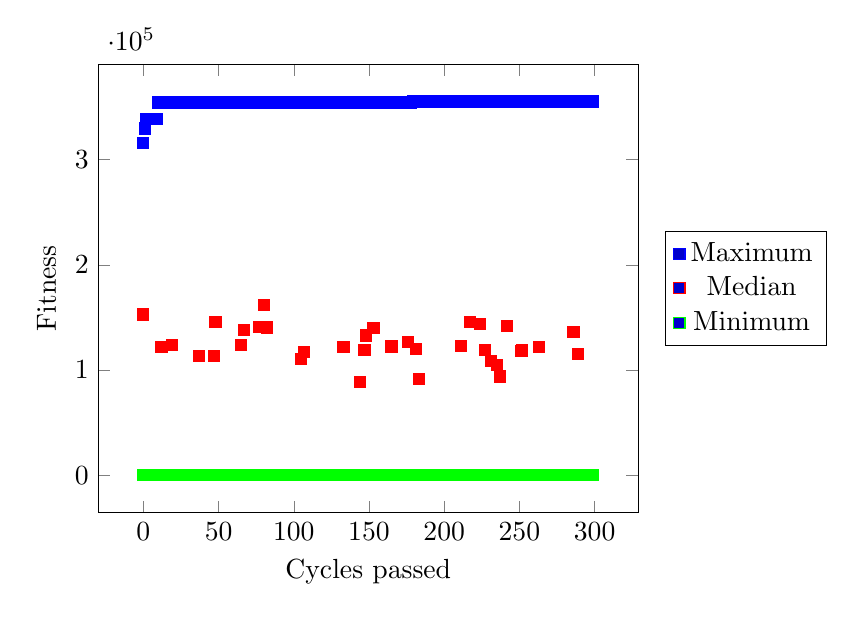
\begin{tikzpicture}
		\begin{axis}[
			xlabel=Cycles passed,
			ylabel=Fitness,
			scatter/classes={
				max={mark=square*,blue},
				med={mark=square*,red},
				min={mark=square*,green}
				}
            ]
            
\addplot+[scatter,only marks,scatter src=explicit symbolic]table[meta=label] {
x y label
0 315921 max
1 329608 max
2 338662 max
3 338662 max
4 338662 max
5 338662 max
6 338662 max
7 338662 max
8 338662 max
9 338662 max
10 354388 max
11 354388 max
12 354388 max
13 354388 max
14 354388 max
15 354388 max
16 354388 max
17 354388 max
18 354388 max
19 354388 max
20 354388 max
21 354388 max
22 354388 max
23 354388 max
24 354388 max
25 354388 max
26 354388 max
27 354388 max
28 354388 max
29 354388 max
30 354388 max
31 354388 max
32 354388 max
33 354388 max
34 354388 max
35 354388 max
36 354388 max
37 354388 max
38 354388 max
39 354388 max
40 354388 max
41 354388 max
42 354388 max
43 354388 max
44 354388 max
45 354388 max
46 354388 max
47 354388 max
48 354388 max
49 354388 max
50 354388 max
51 354388 max
52 354388 max
53 354388 max
54 354388 max
55 354388 max
56 354388 max
57 354388 max
58 354388 max
59 354388 max
60 354388 max
61 354388 max
62 354388 max
63 354388 max
64 354388 max
65 354388 max
66 354388 max
67 354388 max
68 354388 max
69 354388 max
70 354388 max
71 354388 max
72 354388 max
73 354388 max
74 354388 max
75 354388 max
76 354388 max
77 354388 max
78 354388 max
79 354388 max
80 354388 max
81 354388 max
82 354388 max
83 354388 max
84 354388 max
85 354388 max
86 354388 max
87 354388 max
88 354388 max
89 354388 max
90 354388 max
91 354388 max
92 354388 max
93 354388 max
94 354388 max
95 354388 max
96 354388 max
97 354388 max
98 354388 max
99 354388 max
100 354388 max
101 354388 max
102 354388 max
103 354388 max
104 354388 max
105 354388 max
106 354388 max
107 354388 max
108 354388 max
109 354388 max
110 354388 max
111 354388 max
112 354388 max
113 354388 max
114 354388 max
115 354388 max
116 354388 max
117 354388 max
118 354388 max
119 354388 max
120 354388 max
121 354388 max
122 354388 max
123 354388 max
124 354388 max
125 354388 max
126 354388 max
127 354388 max
128 354388 max
129 354388 max
130 354388 max
131 354388 max
132 354388 max
133 354388 max
134 354388 max
135 354388 max
136 354388 max
137 354388 max
138 354388 max
139 354388 max
140 354388 max
141 354388 max
142 354388 max
143 354388 max
144 354388 max
145 354388 max
146 354388 max
147 354388 max
148 354388 max
149 354388 max
150 354388 max
151 354388 max
152 354388 max
153 354388 max
154 354388 max
155 354388 max
156 354388 max
157 354388 max
158 354388 max
159 354388 max
160 354388 max
161 354388 max
162 354388 max
163 354388 max
164 354388 max
165 354388 max
166 354388 max
167 354388 max
168 354388 max
169 354388 max
170 354388 max
171 354388 max
172 354388 max
173 354388 max
174 354388 max
175 354388 max
176 354388 max
177 354388 max
178 354388 max
179 355269 max
180 355269 max
181 355269 max
182 355269 max
183 355269 max
184 355269 max
185 355269 max
186 355269 max
187 355269 max
188 355269 max
189 355269 max
190 355269 max
191 355269 max
192 355269 max
193 355269 max
194 355269 max
195 355269 max
196 355269 max
197 355269 max
198 355269 max
199 355269 max
200 355269 max
201 355269 max
202 355269 max
203 355269 max
204 355269 max
205 355269 max
206 355269 max
207 355269 max
208 355269 max
209 355269 max
210 355269 max
211 355269 max
212 355269 max
213 355269 max
214 355269 max
215 355269 max
216 355269 max
217 355269 max
218 355269 max
219 355269 max
220 355269 max
221 355269 max
222 355269 max
223 355269 max
224 355269 max
225 355269 max
226 355269 max
227 355269 max
228 355269 max
229 355269 max
230 355269 max
231 355269 max
232 355269 max
233 355269 max
234 355269 max
235 355269 max
236 355269 max
237 355269 max
238 355269 max
239 355269 max
240 355269 max
241 355269 max
242 355269 max
243 355269 max
244 355269 max
245 355269 max
246 355269 max
247 355269 max
248 355269 max
249 355269 max
250 355269 max
251 355269 max
252 355269 max
253 355269 max
254 355269 max
255 355269 max
256 355269 max
257 355269 max
258 355269 max
259 355269 max
260 355269 max
261 355269 max
262 355269 max
263 355269 max
264 355269 max
265 355269 max
266 355269 max
267 355269 max
268 355269 max
269 355269 max
270 355269 max
271 355269 max
272 355269 max
273 355269 max
274 355269 max
275 355269 max
276 355269 max
277 355269 max
278 355269 max
279 355269 max
280 355269 max
281 355269 max
282 355269 max
283 355269 max
284 355269 max
285 355269 max
286 355269 max
287 355269 max
288 355269 max
289 355269 max
290 355269 max
291 355269 max
292 355269 max
293 355269 max
294 355269 max
295 355269 max
296 355269 max
297 355269 max
298 355269 max
299 355269 max
};
\addplot+[scatter,only marks,scatter src=explicit symbolic]table[meta=label] {
x y label
0 152738 med
1 0 med
2 0 med
3 0 med
4 0 med
5 0 med
6 0 med
7 0 med
8 0 med
9 0 med
10 0 med
11 0 med
12 121629 med
13 0 med
14 0 med
15 0 med
16 0 med
17 0 med
18 0 med
19 124054 med
20 0 med
21 0 med
22 0 med
23 0 med
24 0 med
25 0 med
26 0 med
27 0 med
28 0 med
29 0 med
30 0 med
31 0 med
32 0 med
33 0 med
34 0 med
35 0 med
36 0 med
37 113357 med
38 0 med
39 0 med
40 0 med
41 0 med
42 0 med
43 0 med
44 0 med
45 0 med
46 0 med
47 113033 med
48 145583 med
49 0 med
50 0 med
51 0 med
52 0 med
53 0 med
54 0 med
55 0 med
56 0 med
57 0 med
58 0 med
59 0 med
60 0 med
61 0 med
62 0 med
63 0 med
64 0 med
65 123526 med
66 0 med
67 137791 med
68 0 med
69 0 med
70 0 med
71 0 med
72 0 med
73 0 med
74 0 med
75 0 med
76 0 med
77 141142 med
78 0 med
79 0 med
80 162005 med
81 0 med
82 140483 med
83 0 med
84 0 med
85 0 med
86 0 med
87 0 med
88 0 med
89 0 med
90 0 med
91 0 med
92 0 med
93 0 med
94 0 med
95 0 med
96 0 med
97 0 med
98 0 med
99 0 med
100 0 med
101 0 med
102 0 med
103 0 med
104 0 med
105 110341 med
106 0 med
107 117163 med
108 0 med
109 0 med
110 0 med
111 0 med
112 0 med
113 0 med
114 0 med
115 0 med
116 0 med
117 0 med
118 0 med
119 0 med
120 0 med
121 0 med
122 0 med
123 0 med
124 0 med
125 0 med
126 0 med
127 0 med
128 0 med
129 0 med
130 0 med
131 0 med
132 0 med
133 121748 med
134 0 med
135 0 med
136 0 med
137 0 med
138 0 med
139 0 med
140 0 med
141 0 med
142 0 med
143 0 med
144 88899 med
145 0 med
146 0 med
147 118694 med
148 132809 med
149 0 med
150 0 med
151 0 med
152 0 med
153 139866 med
154 0 med
155 0 med
156 0 med
157 0 med
158 0 med
159 0 med
160 0 med
161 0 med
162 0 med
163 0 med
164 0 med
165 122428 med
166 0 med
167 0 med
168 0 med
169 0 med
170 0 med
171 0 med
172 0 med
173 0 med
174 0 med
175 0 med
176 126689 med
177 0 med
178 0 med
179 0 med
180 0 med
181 119821 med
182 0 med
183 91239 med
184 0 med
185 0 med
186 0 med
187 0 med
188 0 med
189 0 med
190 0 med
191 0 med
192 0 med
193 0 med
194 0 med
195 0 med
196 0 med
197 0 med
198 0 med
199 0 med
200 0 med
201 0 med
202 0 med
203 0 med
204 0 med
205 0 med
206 0 med
207 0 med
208 0 med
209 0 med
210 0 med
211 122786 med
212 0 med
213 0 med
214 0 med
215 0 med
216 0 med
217 145380 med
218 0 med
219 0 med
220 0 med
221 0 med
222 0 med
223 0 med
224 143636 med
225 0 med
226 0 med
227 118708 med
228 0 med
229 0 med
230 0 med
231 108453 med
232 0 med
233 0 med
234 0 med
235 105037 med
236 0 med
237 93779 med
238 0 med
239 0 med
240 0 med
241 0 med
242 142029 med
243 0 med
244 0 med
245 0 med
246 0 med
247 0 med
248 0 med
249 0 med
250 0 med
251 118194 med
252 118623 med
253 0 med
254 0 med
255 0 med
256 0 med
257 0 med
258 0 med
259 0 med
260 0 med
261 0 med
262 0 med
263 121939 med
264 0 med
265 0 med
266 0 med
267 0 med
268 0 med
269 0 med
270 0 med
271 0 med
272 0 med
273 0 med
274 0 med
275 0 med
276 0 med
277 0 med
278 0 med
279 0 med
280 0 med
281 0 med
282 0 med
283 0 med
284 0 med
285 0 med
286 136411 med
287 0 med
288 0 med
289 115255 med
290 0 med
291 0 med
292 0 med
293 0 med
294 0 med
295 0 med
296 0 med
297 0 med
298 0 med
299 0 med
};
\addplot+[scatter,only marks,scatter src=explicit symbolic]table[meta=label] {
x y label
0 0 min
1 0 min
2 0 min
3 0 min
4 0 min
5 0 min
6 0 min
7 0 min
8 0 min
9 0 min
10 0 min
11 0 min
12 0 min
13 0 min
14 0 min
15 0 min
16 0 min
17 0 min
18 0 min
19 0 min
20 0 min
21 0 min
22 0 min
23 0 min
24 0 min
25 0 min
26 0 min
27 0 min
28 0 min
29 0 min
30 0 min
31 0 min
32 0 min
33 0 min
34 0 min
35 0 min
36 0 min
37 0 min
38 0 min
39 0 min
40 0 min
41 0 min
42 0 min
43 0 min
44 0 min
45 0 min
46 0 min
47 0 min
48 0 min
49 0 min
50 0 min
51 0 min
52 0 min
53 0 min
54 0 min
55 0 min
56 0 min
57 0 min
58 0 min
59 0 min
60 0 min
61 0 min
62 0 min
63 0 min
64 0 min
65 0 min
66 0 min
67 0 min
68 0 min
69 0 min
70 0 min
71 0 min
72 0 min
73 0 min
74 0 min
75 0 min
76 0 min
77 0 min
78 0 min
79 0 min
80 0 min
81 0 min
82 0 min
83 0 min
84 0 min
85 0 min
86 0 min
87 0 min
88 0 min
89 0 min
90 0 min
91 0 min
92 0 min
93 0 min
94 0 min
95 0 min
96 0 min
97 0 min
98 0 min
99 0 min
100 0 min
101 0 min
102 0 min
103 0 min
104 0 min
105 0 min
106 0 min
107 0 min
108 0 min
109 0 min
110 0 min
111 0 min
112 0 min
113 0 min
114 0 min
115 0 min
116 0 min
117 0 min
118 0 min
119 0 min
120 0 min
121 0 min
122 0 min
123 0 min
124 0 min
125 0 min
126 0 min
127 0 min
128 0 min
129 0 min
130 0 min
131 0 min
132 0 min
133 0 min
134 0 min
135 0 min
136 0 min
137 0 min
138 0 min
139 0 min
140 0 min
141 0 min
142 0 min
143 0 min
144 0 min
145 0 min
146 0 min
147 0 min
148 0 min
149 0 min
150 0 min
151 0 min
152 0 min
153 0 min
154 0 min
155 0 min
156 0 min
157 0 min
158 0 min
159 0 min
160 0 min
161 0 min
162 0 min
163 0 min
164 0 min
165 0 min
166 0 min
167 0 min
168 0 min
169 0 min
170 0 min
171 0 min
172 0 min
173 0 min
174 0 min
175 0 min
176 0 min
177 0 min
178 0 min
179 0 min
180 0 min
181 0 min
182 0 min
183 0 min
184 0 min
185 0 min
186 0 min
187 0 min
188 0 min
189 0 min
190 0 min
191 0 min
192 0 min
193 0 min
194 0 min
195 0 min
196 0 min
197 0 min
198 0 min
199 0 min
200 0 min
201 0 min
202 0 min
203 0 min
204 0 min
205 0 min
206 0 min
207 0 min
208 0 min
209 0 min
210 0 min
211 0 min
212 0 min
213 0 min
214 0 min
215 0 min
216 0 min
217 0 min
218 0 min
219 0 min
220 0 min
221 0 min
222 0 min
223 0 min
224 0 min
225 0 min
226 0 min
227 0 min
228 0 min
229 0 min
230 0 min
231 0 min
232 0 min
233 0 min
234 0 min
235 0 min
236 0 min
237 0 min
238 0 min
239 0 min
240 0 min
241 0 min
242 0 min
243 0 min
244 0 min
245 0 min
246 0 min
247 0 min
248 0 min
249 0 min
250 0 min
251 0 min
252 0 min
253 0 min
254 0 min
255 0 min
256 0 min
257 0 min
258 0 min
259 0 min
260 0 min
261 0 min
262 0 min
263 0 min
264 0 min
265 0 min
266 0 min
267 0 min
268 0 min
269 0 min
270 0 min
271 0 min
272 0 min
273 0 min
274 0 min
275 0 min
276 0 min
277 0 min
278 0 min
279 0 min
280 0 min
281 0 min
282 0 min
283 0 min
284 0 min
285 0 min
286 0 min
287 0 min
288 0 min
289 0 min
290 0 min
291 0 min
292 0 min
293 0 min
294 0 min
295 0 min
296 0 min
297 0 min
298 0 min
299 0 min
};

			\addlegendentry{Maximum}
			\addlegendentry{Median}
			\addlegendentry{Minimum}
		\end{axis}
	\end{tikzpicture}
	\caption{Detail of genetic algorithm on balanced data with 30 elements in set and pool size of 300}
\label{plot:genProfile30-pool300}
\end{figure}
